\section{Inspiration Corpus: Pattern Taxonomy}
\label{sec:corpus-taxonomy}

This section analyzes a corpus of technical explainer infographics provided as design inspiration. These images are \emph{not timelines}---they have no time axis. Yet they share visual vocabulary with the timeline engine and reveal the broader grammar family the compiler should support.

\subsection{The Corpus}

Sixteen technical infographics from the ByteByteGo-style AI-engineering and
developer content space, organized by visual pattern:

\begin{enumerate}
  \item \textbf{10x-coding-playbook}: Multi-section poster about parallel AI
        coding workflows (timeline + step-cards + stats)
  \item \textbf{rag-vectorless-explainer}: Step-by-step explanation of
        vectorless RAG (flow + tree + step-cards + stats)
  \item \textbf{dsa-patterns-grid}: Grid of algorithm pattern visualizations
        (comparison/matrix kind)
  \item \textbf{claude-vs-openclaw-matrix}: Feature comparison matrix between
        two AI agents (comparison/matrix kind)
  \item \textbf{calculator-vs-ai}: Two-column comparison with stats
        (comparison/matrix kind)
  \item \textbf{agent-harness}: Hub-and-spoke architecture diagram
        (node-link/topology kind)
  \item \textbf{archon-harness-builder}: Multi-section poster with timeline,
        stats, flow, and comparison elements
  \item \textbf{openclaw-vps-architecture}: Nested container architecture
        diagram with external connections (node-link/topology kind)
  \item \textbf{single-vs-multi-agent}: Stacked node-link diagrams
        (node-link/topology kind)
  \item \textbf{explainer-01} through \textbf{explainer-16}: Sixteen
        ByteByteGo-style technical explainer infographics covering the full
        taxonomy: pipeline/sequence diagrams with animated arrow cues,
        step-card sequences, comparison/matrix grids, stat callouts,
        swimlane timelines, and multi-panel poster compositions.
\end{enumerate}

Figure~\ref{fig:corpus-10x} shows a multi-pattern poster; Figure~\ref{fig:corpus-rag}
shows a RAG pipeline explainer.
Figure~\ref{fig:corpus-explainer} shows a representative ByteByteGo-style
explainer from the extended corpus.

\begin{figure}[h]
\centering
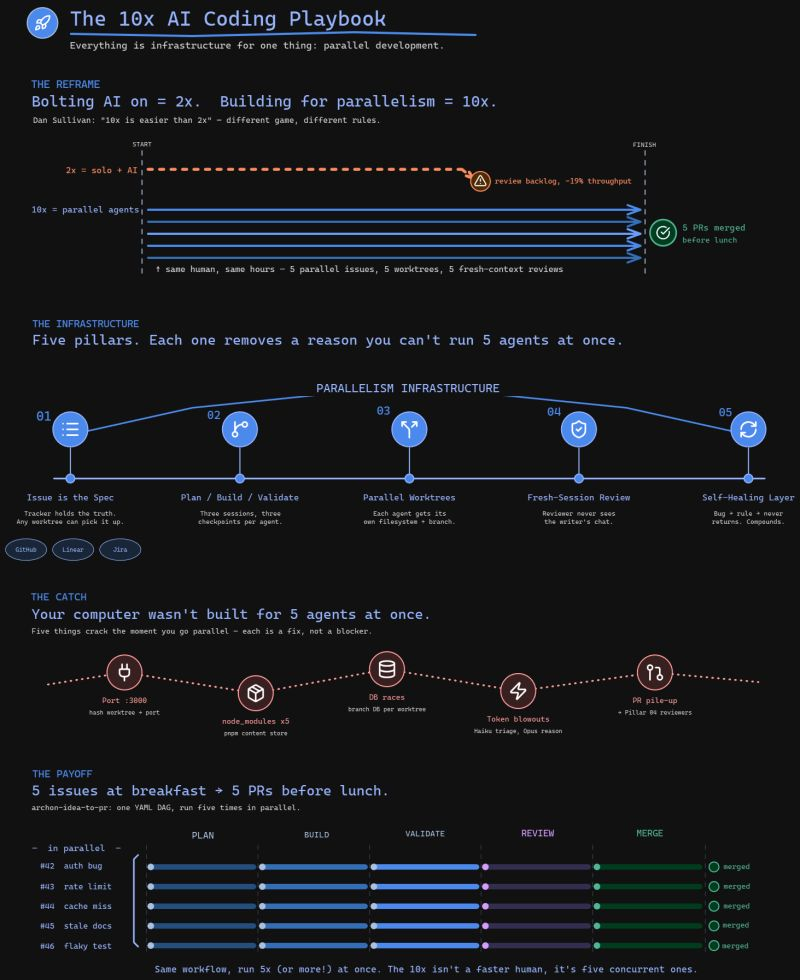
\includegraphics[width=0.95\linewidth]{figures/corpus/10x-coding-playbook.png}
\caption{10x AI Coding Playbook: A multi-section poster combining timeline-like horizontal bars, numbered step-cards with icons, flow pipelines, and stat callouts. Note the swimlane structure in ``THE PAYOFF'' section---this is the timeline engine's horizontal layout.}
\label{fig:corpus-10x}
\end{figure}

\begin{figure}[h]
\centering
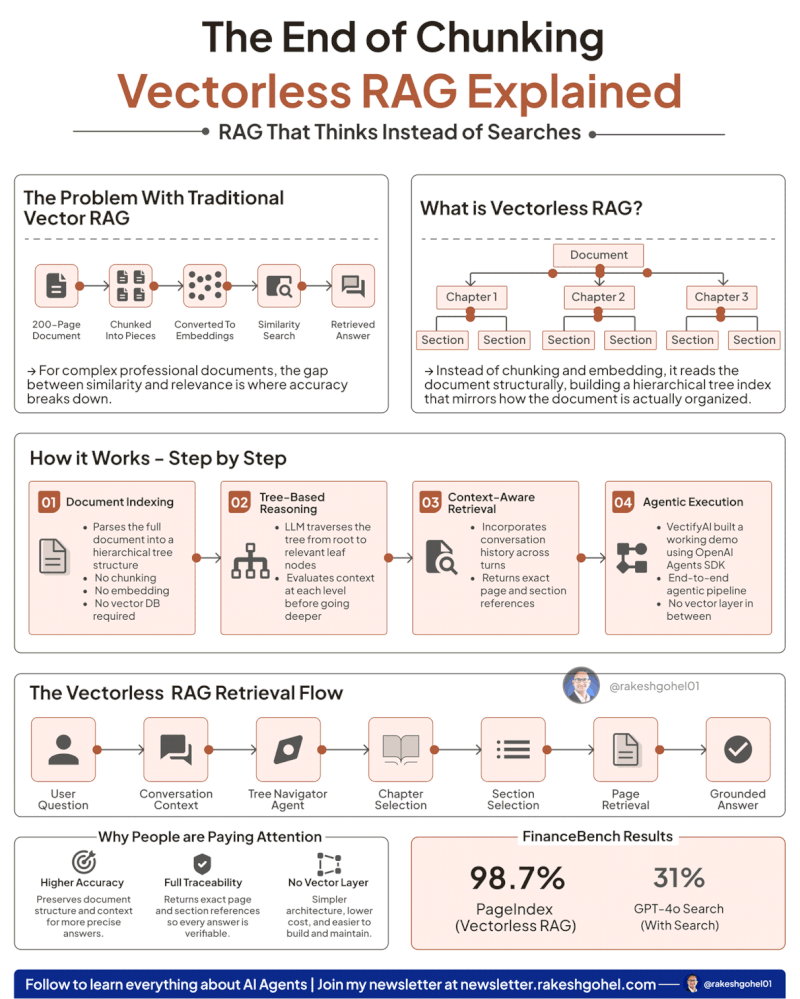
\includegraphics[width=0.95\linewidth]{figures/corpus/rag-vectorless-explainer.png}
\caption{Vectorless RAG Explainer: Combines flow/pipeline (top left, bottom), tree diagram (top right), numbered step-cards (middle), stat callouts (bottom right), and section-stacked poster composition.}
\label{fig:corpus-rag}
\end{figure}

\begin{figure}[h]
\centering
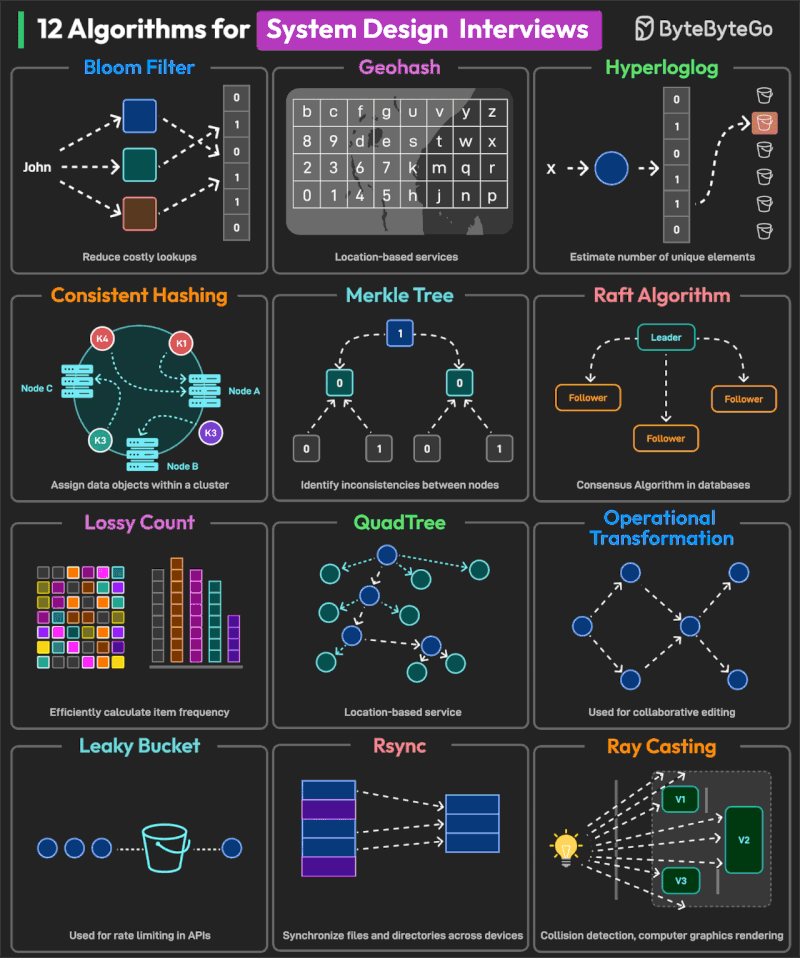
\includegraphics[width=0.80\linewidth]{figures/corpus/explainer-05-d6bdbd.png}
\caption{ByteByteGo-style technical explainer (corpus image 05). Representative of the pipeline/sequence kind with numbered steps, annotated arrows, and stat callouts. The animated-arrow variant of this kind (flowing dashes along connector paths) is a recurring motif in the extended corpus.}
\label{fig:corpus-explainer}
\end{figure}

\subsection{Extracted Visual Vocabulary}

Analysis reveals recurring diagram kinds that form a taxonomy:

\subsubsection{Node-Link Graph}

\textbf{Description:} Vertices (circles, icons, or labeled boxes) connected by edges (lines, arrows). Includes trees, networks, hub-and-spoke patterns, and architecture diagrams.

\textbf{Corpus examples:}
\begin{itemize}
  \item Tree structure in rag-vectorless-explainer (``Document'' → ``Chapter'' → ``Section'')
  \item Hub-and-spoke in agent-harness (AI Model at center, tools radiating out)
  \item Network in single-vs-multi-agent (agent nodes connected by edges)
  \item Nested containers in openclaw-vps-architecture
\end{itemize}

\textbf{Layout challenge:} General 2D graph auto-layout is research-grade. Practical approach: opinionated layout per sub-kind (tidy-tree, left-right pipeline, hub-and-spoke, swimlane).

\subsubsection{Flow/Pipeline (including Animated-Arrow Variant)}

\textbf{Description:} Ordered sequence of icon+label nodes connected by arrows. May include branches, loops, and legends. The dominant idiom for explaining processes.

\textbf{Corpus examples:}
\begin{itemize}
  \item ``The Vectorless RAG Retrieval Flow'' (rag-vectorless-explainer, bottom)
  \item ``ONE WORKFLOW. ONE YAML FILE.'' (archon-harness-builder, middle)
  \item ``The Problem With Traditional Vector RAG'' (rag-vectorless-explainer, top-left)
  \item Multiple explainers (explainer-03, explainer-07, explainer-11): pipeline
        steps with dashed-line or colored-border connectors suggesting
        sequential activation.
\end{itemize}

\textbf{Key observation:} Flow pipelines are essentially timeline milestone-nodes + connectors + icons \emph{minus the time axis}. Most of the rendering logic is reusable.

\medskip\noindent
\textbf{Animated-arrow variant.}
Several corpus images (particularly in the ByteByteGo extended set) show
connector arrows with dashed or pulsing aesthetics that strongly imply
motion --- data flowing through a pipeline, a request propagating through
a system.  In the SVG animation layer, this maps to
\texttt{stroke-dashoffset} animation on the connector path:
a CSS keyframe or SMIL \texttt{<animate>} element that advances the dash
offset at a fixed rate produces the ``flowing'' effect.
This is a first-class animation pattern for the Flow grammar and does not
require any changes to the static Scene IR --- only an animation hint attached
to the connector's path element.

\subsubsection{Numbered Step-Cards}

\textbf{Description:} Ordinal number + icon + title + bullet points in a card. Used for step-by-step explanations.

\textbf{Corpus examples:}
\begin{itemize}
  \item ``How it Works -- Step by Step'' (rag-vectorless-explainer): 4 numbered cards
  \item ``THE INFRASTRUCTURE'' (10x-coding-playbook): 5 numbered circular icons with labels
\end{itemize}

\textbf{Key observation:} The numbered-step arcs in 10x-coding-playbook are literally the timeline's numbered milestone nodes on a horizontal axis with connecting lines.

\subsubsection{Comparison (Matrix/Table)}
\label{sec:corpus-comparison-matrix}

\textbf{Description:} $N$ columns (or rows) comparing items across features.
Cells contain checkmarks, $\times$ marks, stats, or feature descriptions.
This is a \emph{genuinely tabular} kind --- not a flow, not a graph ---
where columns are items, rows are attributes, and cells encode presence,
absence, or magnitude.
It is structurally orthogonal to all flow-derived diagram kinds: there is
no directed-edge concept, no time axis, and no positional encoding of
ordering beyond row/column position.

\textbf{Corpus examples:}
\begin{itemize}
  \item claude-vs-openclaw-matrix: 2 columns, 5 feature rows with icons
  \item calculator-vs-ai: 2 columns with hero images and stat rows
  \item dsa-patterns-grid: 15 algorithm pattern cells in a 5$\times$3 grid
        (each cell is a mini diagram + label --- a grid of comparison cells)
  \item ``THE PROBLEM'' / ``Archon -- The Harness'' (archon-harness-builder):
        side-by-side comparison columns
  \item explainer-04 (corpus extended): 3-column capability comparison with
        checkmark/X indicator cells
\end{itemize}

\textbf{Grammar design note.}
The Comparison grammar must be kept separate from the Flow/Pipeline grammar.
Its layout is a constrained-grid assignment (column widths auto-computed from
cell content; row heights from maximum cell height in the row) rather than a
directed-graph algorithm.
The primitive unit is a \emph{cell} (possibly containing an icon, a stat, a
description string, or a checkmark indicator), not a \emph{node with edges}.
Conflating comparison with flow in a single grammar would violate the
two-IR-layer principle of semantic tightness.

\subsubsection{Stat Callout}

\textbf{Description:} Large number (``98.7\%'', ``6.7\% → 68.3\%'', ``1,300 PRs/week'') with caption text. Used for impact/results communication.

\textbf{Corpus examples:}
\begin{itemize}
  \item ``FinanceBench Results'' (rag-vectorless-explainer): ``98.7\%'' and ``31\%'' stats
  \item ``WHY HARNESSES MATTER'' (archon-harness-builder): three stat callouts
\end{itemize}

\subsubsection{Array/Cells/Table/Matrix}

\textbf{Description:} Grid of cells, often with indices or labels. Used for data structure visualizations.

\textbf{Corpus examples:}
\begin{itemize}
  \item dsa-patterns-grid: 15 algorithm pattern cells in a grid
  \item Array visualizations within dsa-patterns-grid (Prefix Sum, Two Pointers, etc.)
\end{itemize}

\subsubsection{Swimlane/Gantt}

\textbf{Description:} Horizontal lanes with bars or nodes positioned along a (possibly implicit) time or sequence axis.

\textbf{Corpus examples:}
\begin{itemize}
  \item ``THE PAYOFF'' (10x-coding-playbook): 5 parallel tracks with milestone dots
  \item ``THE REFRAME'' (10x-coding-playbook): 2 horizontal bar timelines
\end{itemize}

\textbf{Key observation:} This \emph{is} the timeline grammar. The corpus validates that the timeline engine's horizontal swimlane layout appears in non-timeline contexts.

\subsubsection{Nested Containers}

\textbf{Description:} Boxes within boxes representing containment (VPS → Container → Components).

\textbf{Corpus examples:}
\begin{itemize}
  \item openclaw-vps-architecture: Hetzner VPS → Docker Container → internal components
\end{itemize}

\subsubsection{Section-Stacked Poster Composition}

\textbf{Description:} Multiple sections stacked vertically, each with a title and distinct content. The overall composition is a poster or long-form infographic.

\textbf{Corpus examples:}
\begin{itemize}
  \item 10x-coding-playbook: 4 sections (THE REFRAME, THE INFRASTRUCTURE, THE CATCH, THE PAYOFF)
  \item archon-harness-builder: 4 sections with different diagram types
  \item rag-vectorless-explainer: 5 logical sections
\end{itemize}

\subsubsection{Editorial Chrome}

\textbf{Description:} Title hierarchy, dividers, legends, footer/branding, author badges. Not content diagrams, but structural framing.

\textbf{Corpus examples:}
\begin{itemize}
  \item All corpus images have prominent titles, subtitles, and section headers
  \item rag-vectorless-explainer: author avatar and handle (``@rakeshgohel01'')
  \item archon-harness-builder: branded logo/icon
  \item 10x-coding-playbook: pill-shaped badges (``GitHub'', ``Linear'', ``Jira'')
\end{itemize}

\subsection{Key Observation: Reuse Potential}

Several corpus patterns are \textbf{already expressible} with the timeline engine's existing primitives:

\begin{itemize}
  \item \textbf{Horizontal swimlanes} (THE PAYOFF, THE REFRAME) = timeline horizontal layout
  \item \textbf{Numbered step arcs} (THE INFRASTRUCTURE) = milestones with ordinal labels + connectors
  \item \textbf{Flow pipelines} = milestone nodes + connectors + icons, no time axis
  \item \textbf{Stat callouts} = text primitives with large font size
  \item \textbf{Editorial chrome} = metadata (title, subtitle), legend, theme styling
\end{itemize}

The genuinely \textbf{new work} required:

\begin{enumerate}
  \item \textbf{Node-link graph layout}: Tree layout (Reingold-Tilford~\cite{reingold1981}), DAG layout (Sugiyama~\cite{sugiyama1981}), hub-and-spoke
  \item \textbf{Multi-panel composition}: Arranging multiple grammar outputs into a poster
  \item \textbf{Comparison grammar}: Column/row structure with indicator cells
  \item \textbf{Container nesting}: Recursive group layout for architecture diagrams
\end{enumerate}

\subsection{Grammar Sequencing Recommendation}

Based on corpus analysis, the recommended grammar implementation order is:

\begin{enumerate}
  \item \textbf{Timeline} (done): Horizontal swimlane, vertical spine, serpentine
  \item \textbf{Flow/Pipeline} (next): Maximum reuse of nodes/connectors/icons; natural home for animation (flowing arrows); cheapest new grammar
  \item \textbf{Comparison}: Column/row structure; relatively simple layout
  \item \textbf{Stat Callout}: Trivial layout (large text); cheap win
  \item \textbf{Node-Link Graph}: Highest leverage, hardest layout (requires auto-layout algorithms)
  \item \textbf{Composition}: Assembles multiple panels into posters; depends on other grammars
\end{enumerate}
